\section{CREAR RELACIONES} 
\subsection {TAREA 1:  RELACIONES AUTOMATICAS}

\begin{itemize}

\item 1. Iniciar Power BI Desktop.
\item 2. En la Ventana de Power BI Desktop, click en Obtener Datos (Get Data).
\item 3. En el cuadro de dialogo Obtener Datos (Get Data), asegurarse que Excel esta seleccionado y hacer click en Conectar (Connect). \\
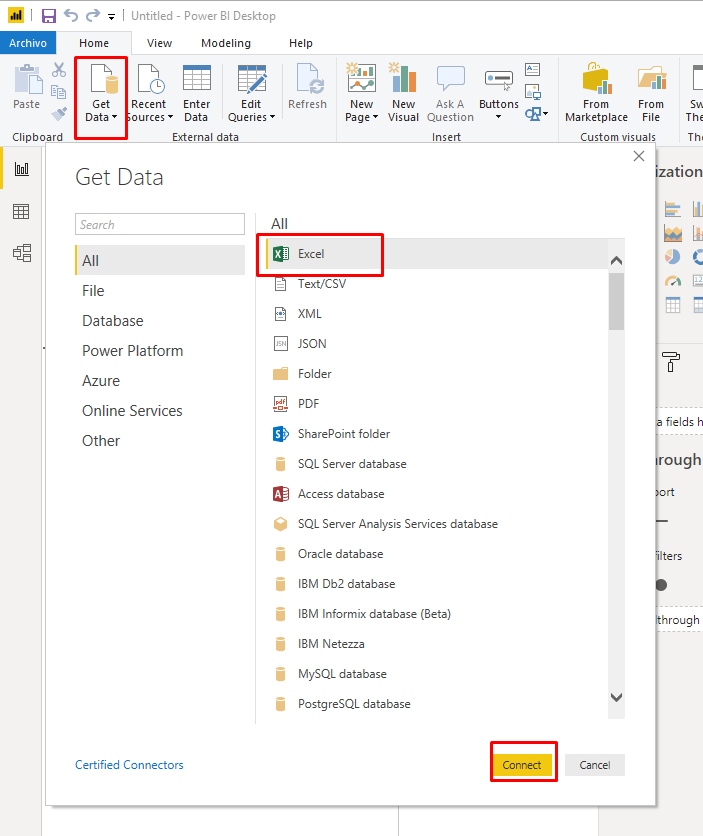
\includegraphics[scale=0.5]{./Imagenes/image001}
\item 4. En el cuadro de dialogo Abrir (Open), buscar el archivo Adventure Works Sales Data.xlsx, y luego hacer click en Abrir (Open).
\item 5. En el cuadro de dialogo Explorador (Navigator), seleccionar las hojas DimCurrency, DimCustomer,DimDate, DimProduct, DimPromotion, DimSalesTerritory, y FactInternetSales.
\item 6. Hacer click en Cargar (Load). \\
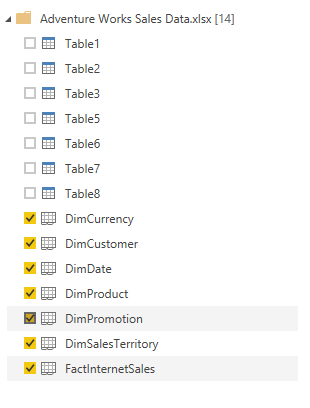
\includegraphics[scale=0.5]{./Imagenes/image002}
\item 7.En el panel de vistas a mano derecho, hacer click en Relaciones (Relationships).
\item 8.En el menú principal, hacer click en Administrar relaciones (Manage Relationships).
\item 9. En el cuadro de Administrar relaciones (Manage Relationships), hacer click en Nueva (New). \\
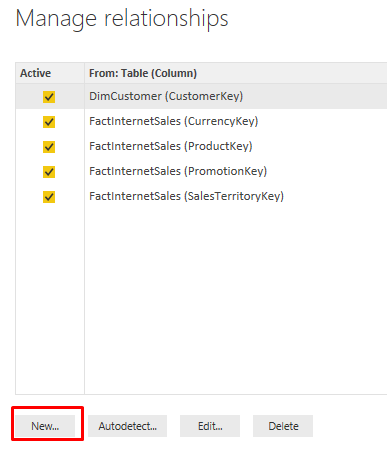
\includegraphics[scale=0.5]{./Imagenes/image003}
\item 10.En el cuadro de Administrar relaciones (Manage Relationships), en la lista de tablas superior, hacer click en FactInternetSales. Cuando la vista previa de la table aparezca hacer click en la columna OrderDateKey.
\item 11. En la lista de table inferior, hacer click en DimDate. Cuando la vista previa de la table aparezca hacer click en la columna DateKey.
\item 12. Revisar que la cardinalidad (Cardinality) esta seleccionada para Muchos a Uno (Many to One (*:1)), que la Dirección del filtro cruzado (Cross filter direction) es Sencilla (Single), y que la opción Hacer esta relaciónactiva (Make this relationship active) se encuentra seleccionada, luego hacer click en Aceptar (OK).
\item 13. En el cuadro de Administrar relaciones (Manage Relationships), hacer click en Cerrar (Close). \\
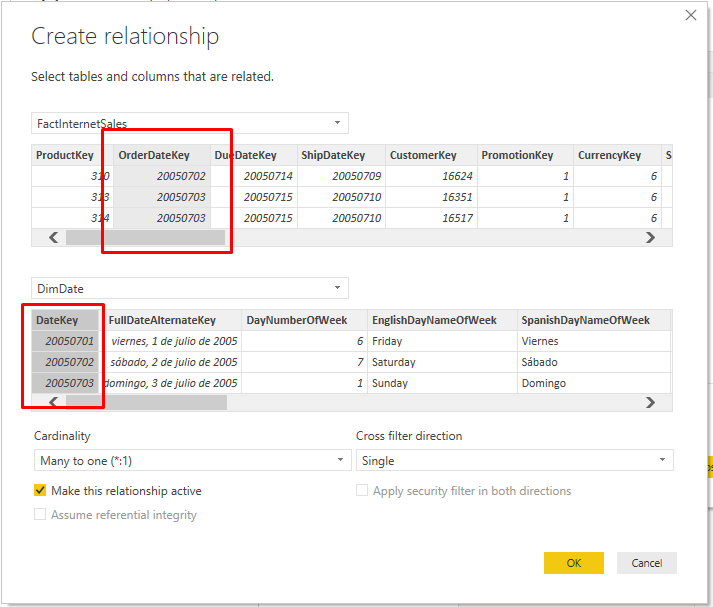
\includegraphics[scale=0.5]{./Imagenes/image004}
\item 14.En el diagrama, en la tabla FactInternetSales, hacer click en la columna DueDateKey. Arrastrar la columna DueDateKey a la columna DateKey de la tabla DimDate.
\item 15. En el diagrama, en la tabla FactInternetSales, hacer click en la columna ShipDateKey. Arrastrar la columna ShipDateKey a la columna DateKey de la tabla DimDate. \\
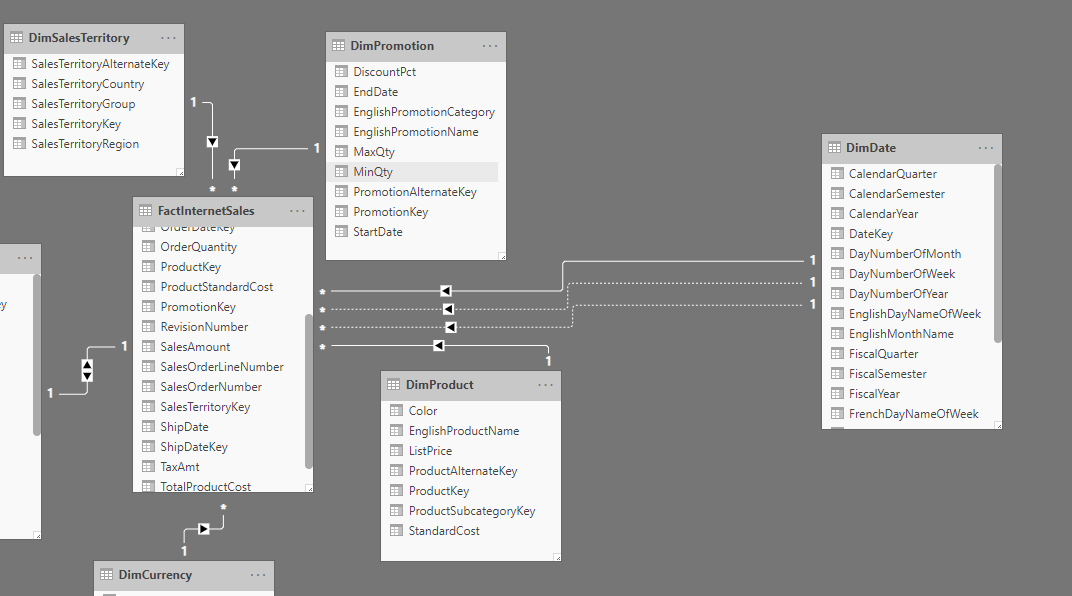
\includegraphics[scale=0.5]{./Imagenes/image005}
\item 16. En el menú principal, hacer click en Administrar relaciones (Manage Relationships).
\item 17. En el cuadro de Administrar relaciones (Manage Relationships), hacer doble click en la relación FactInternetSales (CurrencyKey). \\
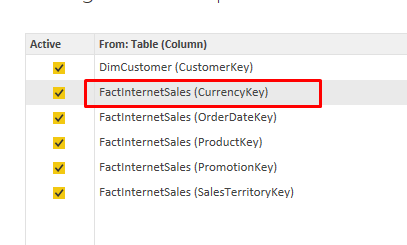
\includegraphics[scale=0.5]{./Imagenes/image006}
\item 18. En la lista de Dirección de Filtro Cruzado (Cross filter direction), hacer click en Sencilla (Single), luego hacer click en Aceptar (OK).
\item 19. En el cuadro de Administrar relaciones (Manage Relationships), hacer doble click en la relación FactInternetSales (ProductKey).
\item 20. En la lista de Dirección de Filtro Cruzado (Cross filter direction), hacer click en Sencilla (Single), luego hacer click en Aceptar (OK).
\item 21. En el cuadro de Administrar relaciones (Manage Relationships), hacer doble click en la relación FactInternetSales (PromotionKey).
\item 22. En la lista de Dirección de Filtro Cruzado (Cross filter direction), hacer click en Sencilla (Single), luego hacer click en Aceptar (OK).\\
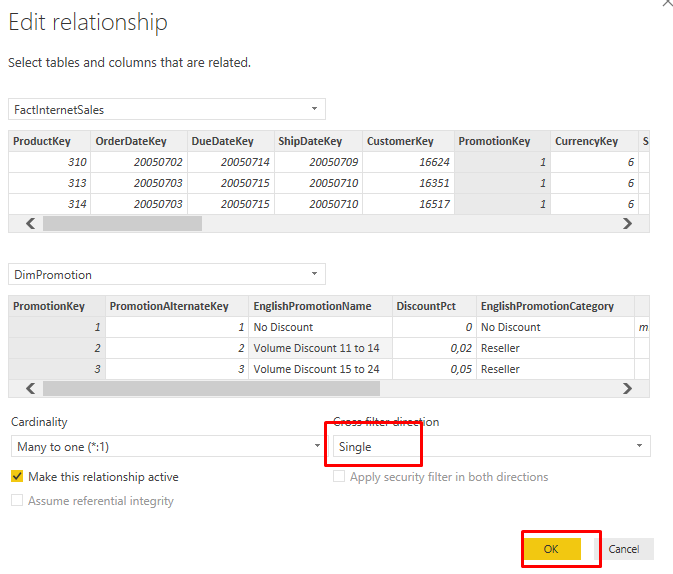
\includegraphics[scale=0.5]{./Imagenes/image007}
\item 23. En el cuadro de Administrar relaciones (Manage Relationships), hacer doble click en la relación FactInternetSales (SalesTerritoryKey).
\item 24. En la lista de Dirección de Filtro Cruzado (Cross filter direction), hacer click en Sencilla (Single), luego hacer click en Aceptar (OK). \\
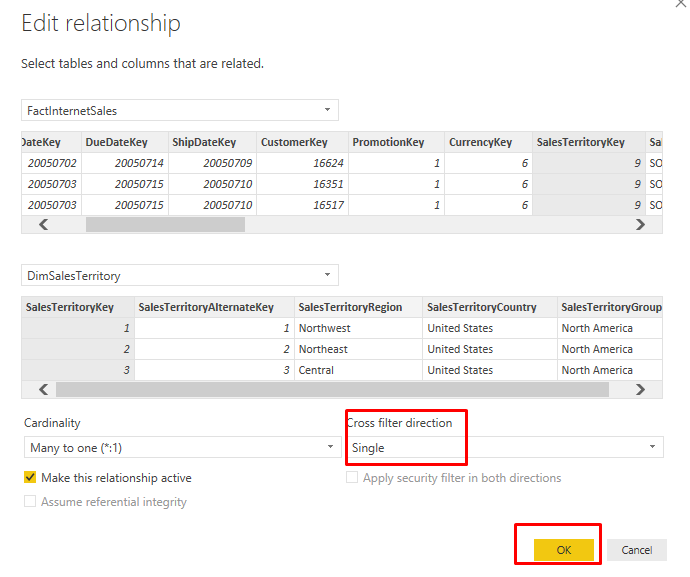
\includegraphics[scale=0.5]{./Imagenes/image008}
\item 25. En el cuadro de Administrar relaciones (Manage Relationships), hacer click en Cerrar (Close)..
\item 26. Hacer click en la línea de relación entre FactInternetSales and DimCustomer y presionar Borrar (Delete).
\item 27. En el cuadro de dialogo Eliminar relación (Delete Relationship), hacer click en Borrar (Delete).\\
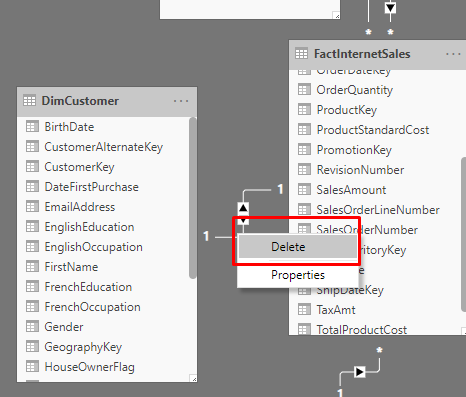
\includegraphics[scale=0.5]{./Imagenes/image009}
\item 28. En el menú principal, hacer click en Administrar relaciones (Manage Relationships).
\item 29. En el cuadro de Administrar relaciones (Manage Relationships), hacer click en Nueva (New).
\item 30. En la lista de tablas superior, hacer click en FactInternetSales. Luego hacer click en la columna CustomerKey en la vista de datos previa.
\item 31. En la lista de tablas superior, hacer click en DimCustomer, y hacer click CustomerKey en la vista de datos previa.
\item 32. En la lista de Cardinalidad (Cardinality), hacer click en Muchos a Uno (Many to One (*:1)), y luego hacer click en Aceptar (OK). \\
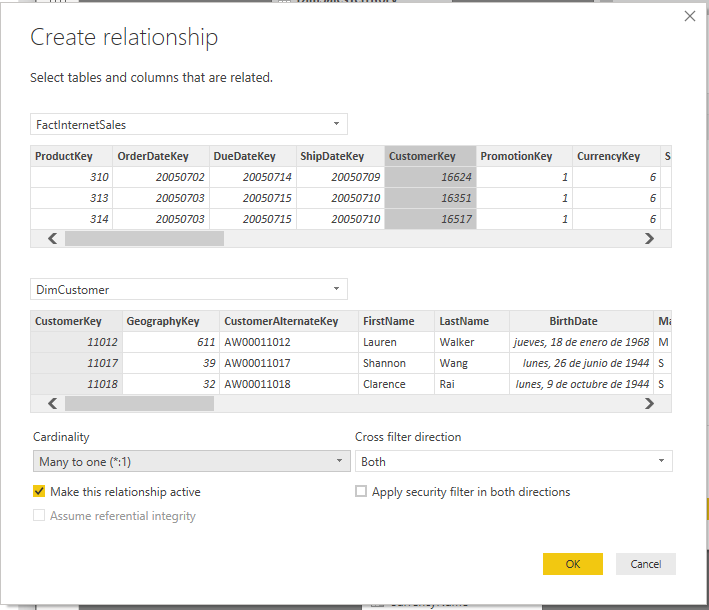
\includegraphics[scale=0.5]{./Imagenes/image010}
\item 33. En el cuadro de Administrar relaciones (Manage Relationships), hacer click en Cerrar (Close).
\item 34. Hacer click en Guardar (Save), y cuargar el archive como Ventas Adventure Works.pbix.\\
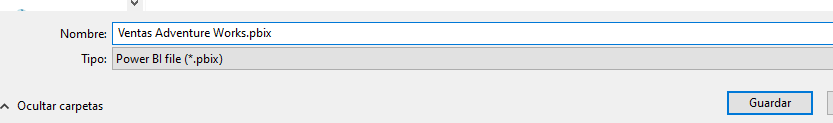
\includegraphics[scale=0.5]{./Imagenes/image011}

\subsection {TAREA 2:  RELACIONES MANUALES}
\item 1. En la Ventana de Power BI Desktop, click en Obtener Datos (Get Data) y luego en Excel
\item 2. Abrir el archivo Adventure Works Product Categories.xlsx.
\item 3. En el cuadro de dialogo Explorador (Navigator), seleccionar las hojas DimProductCategory, andDimProductSubcategory, y luego hacer click en Cargar (Load).\\
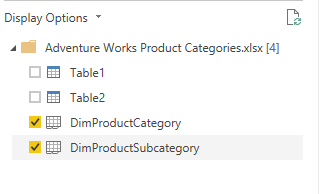
\includegraphics[scale=0.5]{./Imagenes/image012}
\item 4. En el panel de Relaciones, revisar la relación que Power BI ha creado entre las dos tablas.
\item 5. Hacer click en la línea de la relación entre DimProductCategory, y DimProductSubcategory, y seleccionar Eliminar (Delete). \\
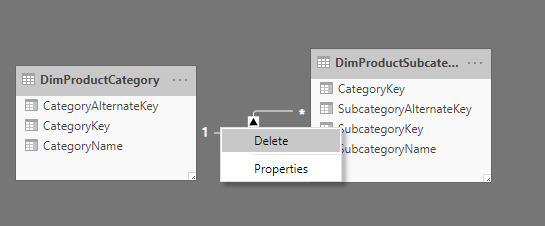
\includegraphics[scale=0.5]{./Imagenes/image013}
\item 6. En el cuadro de dialogo Eliminar relación (Delete Relationship), hacer click en Borrar (Delete).
\item7. Arrastrar la columna CategoryKey en la tabla DimProductSubcategory a la columna Category en la tabla DimProductCategory, para crear una relación Muchos a uno (Many to One (*:1)), y una dirección de filtro cruzado (Cross filter direction) en ambos.
\item 8. En la tabla DimProduct, arrastrar la columna ProductSubcategoryKey a la columna SubcategoryKey en la tabla DimProductSubcategory, para crear una relación de Muchos a Uno (Many to One (*:1)), y una dirección de filtro cruzado (Cross filter direction) en ambos.
\item9. Hacer click en Guardar \\
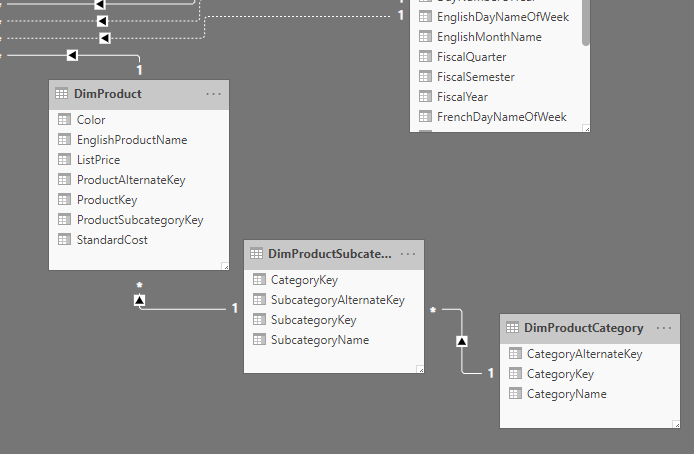
\includegraphics[scale=0.5]{./Imagenes/image014}


\end{itemize}